\section{More experiment results}

% \todo{Method name}

\subsection{Training longer}
As shown in Figure~\ref{fig:Longer-training}, We show that our method can maintain the robust test accuracy with more training epochs. Here, we follow the settings in Figure~\ref{fig:mitigate-overfitting} except we train for additional epochs up to $400$ epochs for each dataset.

\begin{figure*}[t]
  \centering
  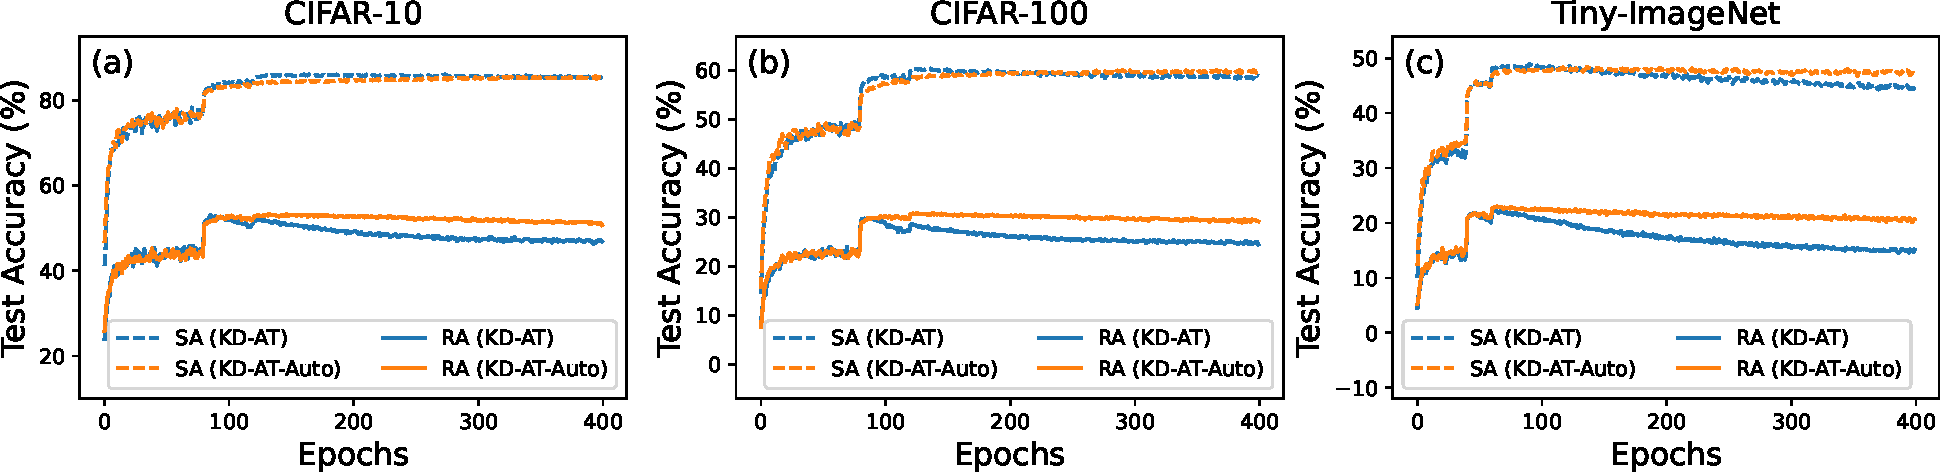
\includegraphics[width=0.98\linewidth]{figures/longer-training.pdf}
  \vspace{-1ex}
  \caption{Our method can maintain robust test accuracy for more training epochs. 
  }
\label{fig:Longer-training}
% \vspace{-2ex}
\end{figure*}



\subsection{Adversarial training methods, neural architectures and evaluation metrics}
\label{sect:more-result}

In this section we conduct extensive experiments with different neural architectures, adversarial training methods and robustness evaluation metrics to verify the effectiveness of our method.



% -------------- Models ----------------
\begin{table*}[!ht]
  \small
  \caption{Performance of our method with different neural architectures.
   }
  \vspace{0.5ex}
  \label{table:result-model}
  \centering
  \small
  \begin{tabular}{clcccccccc}
    \toprule
    \multirow{2}{*}{Architecture} & \multirow{2}{*}{Setting} & \multirow{2}{*}{$T$} & \multirow{2}{*}{$\lambda$} & \multicolumn{3}{c}{Robust Acc. (\%)} & \multicolumn{3}{c}{Standard Acc. (\%)}\\
     & & &  & Best & Last & Diff. & Best & Last & Diff.\\
%     \midrule
% \multirow{3}{*}{pre-act ResNet-18} & Baseline & - & - &  $47.35$ & $41.42$ & $ 5.93$ &  $82.67$ &  $84.91$ & $-2.24$ \\
%  & KD & $2$ & $0.5$ &  $48.76$ & $46.33$ & $ 2.43$ &  $82.89$ &  $85.49$ & $-2.60$ \\ 
%  & KD & $1.47^*$ & $0.8^*$ &  $49.05$ & $48.80$ & $ 0.25$ &  $84.26$ &  $84.47$ & $-0.21$ \\ 
    \midrule
\multirow{3}{*}{VGG-19} 
& AT & - & - &  $42.21$ & $39.12$ & $ 3.09$ &  $73.95$ &  $80.45$ & -$6.50$ \\ 
& KD-AT & $2$ & $0.5$ &  $43.59$ & $42.69$ & $ 0.90$ &  $74.30$ &  $\textbf{77.80}$ & -$3.50$ \\ 
& KD-AT-Auto & $1.28^*$ & $0.79^*$ &  $\textbf{44.27}$ & $\textbf{44.24}$ & $ \textbf{0.03}$ &  $\textbf{76.41}$ &  $76.79$ & $\textbf{-0.38}$ \\ 
    \midrule
\multirow{3}{*}{WRN-28-5} 
& AT & - & - &  $49.85$ & $42.89$ & $ 6.96$ &  $84.82$ &  $85.87$ & -$1.05$ \\ 
& KD-AT & $2$ & $0.5$ &  $51.08$ & $48.40$ & $ 2.68$ &  $85.36$ &  $\textbf{86.88}$ & -$1.52$ \\ 
& KD-AT-Auto & $1.6^*$ & $0.82^*$ &  $\textbf{51.47}$ & $\textbf{51.10}$ & $\textbf{0.37}$ &  $\textbf{86.05}$ &  $86.24$ & $\textbf{-0.19}$ \\ 
    \midrule
\multirow{3}{*}{WRN-34-10} 
& AT & - & - &  $52.29$ & $46.04$ & $ 6.25$ &  $86.57$ &  $86.75$ & -$0.18$ \\ 
& KD-AT & $2$ & $0.5$ &  $53.11$ & $50.97$ & $ 2.14$ &  $86.41$ &  $\textbf{88.06}$ & -$1.65$ \\ 
& KD-AT-Auto & $1.6^*$ & $0.83^*$ &  $\textbf{54.17}$ & $\textbf{53.71}$ & $\textbf{0.46}$ &  $\textbf{87.69}$ &  $88.01$ & $\textbf{-0.32}$ \\ 
    \bottomrule
    % \tablefootnote{$^*$ indicates the best hyper-parameter searched.}
  \end{tabular}
\end{table*}


% -------------- Methods ----------------
\begin{table*}[!ht]
  \small
  \caption{Performance of our method with different adversarial training methods. 
   }
  \vspace{0.5ex}
  \label{table:result-method}
  \centering
  \small
  \begin{tabular}{clcccccccc}
    \toprule
    \multirow{2}{*}{Method} & \multirow{2}{*}{Setting} & \multirow{2}{*}{$T$} & \multirow{2}{*}{$\lambda$} & \multicolumn{3}{c}{Robust Acc. (\%)} & \multicolumn{3}{c}{Standard Acc. (\%)}\\
     & & &  & Best & Last & Diff. & Best & Last & Diff.\\
%     \midrule
% \multirow{3}{*}{PGD} & Baseline & - & - &  $47.35$ & $41.42$ & $ 5.93$ &  $82.67$ &  $84.91$ & -$2.24$ \\
%  & KD & $2$ & $0.5$ &  $48.76$ & $46.33$ & $ 2.43$ &  $82.89$ &  $\textbf{85.49}$ & -$2.60$ \\ 
%  & KD & $1.47^*$ & $0.8^*$ &  $\textbf{49.05}$ & $\textbf{48.80}$ & $ \textbf{0.25}$ &  $\textbf{84.26}$ &  $84.47$ & $\textbf{-0.21}$ \\ 
    \midrule
\multirow{3}{*}{TRADES} 
& AT & - & - &  $48.50$ & $45.53$ & $ 2.97$ &  $82.79$ &  $82.68$ & $ 0.11$ \\ 
& KD-AT & $2$ & $0.5$ &  $48.74$ & $47.52$ & $ 1.22$ &  $82.30$ &  $\textbf{83.03}$ & -$0.73$ \\ 
& KD-AT-Auto & $1.12^*$ & $0.82^*$ &  $\textbf{48.75}$ & $\textbf{48.39}$ & $ \textbf{0.36}$ &  $\textbf{82.44}$ &  $82.80$ & $\textbf{-0.36}$ \\ 
    \midrule
\multirow{3}{*}{FGSM}
& AT & - & - &  $41.96$ & $35.39$ & $ 6.57$ &  $85.91$ &  $87.20$ & -$1.29$ \\ 
& KD-AT & $2$ & $0.5$ &  $42.82$ & $41.61$ & $ 1.21$ &  $86.69$ &  $\textbf{87.93}$ & -$1.24$ \\ 
& KD-AT-Auto & $2.18^*$ & $0.78^*$ &  $\textbf{44.11}$ & $\textbf{43.75}$ & $ \textbf{0.36}$ &  $\textbf{87.38}$ &  $87.66$ & $\textbf{-0.28}$ \\ 

    \bottomrule
    % \tablefootnote{$^*$ indicates the best hyper-parameter searched.}
  \end{tabular}
\end{table*}




% % -------------- Models ----------------
% \begin{table*}[!ht]
%   \small
%   \caption{Performance of our method with different neural architectures.
%   }
%   \vspace{0.5ex}
%   \label{table:result-model}
%   \centering
%   \small
%   \begin{tabular}{clcccccccc}
%     \toprule
%     \multirow{2}{*}{Architecture} & \multirow{2}{*}{Setting} & \multirow{2}{*}{$T$} & \multirow{2}{*}{$\lambda$} & \multicolumn{3}{c}{Robust Acc. (\%)} & \multicolumn{3}{c}{Standard Acc. (\%)}\\
%      & & &  & Best & Last & Diff. & Best & Last & Diff.\\
% %     \midrule
% % \multirow{3}{*}{pre-act ResNet-18} & Baseline & - & - &  $47.35$ & $41.42$ & $ 5.93$ &  $82.67$ &  $84.91$ & $-2.24$ \\
% %  & KD & $2$ & $0.5$ &  $48.76$ & $46.33$ & $ 2.43$ &  $82.89$ &  $85.49$ & $-2.60$ \\ 
% %  & KD & $1.47^*$ & $0.8^*$ &  $49.05$ & $48.80$ & $ 0.25$ &  $84.26$ &  $84.47$ & $-0.21$ \\ 
%     \midrule
% \multirow{3}{*}{VGG-19} 
% & AT & - & - &  $42.21$ & $39.12$ & $ 3.09$ &  $73.95$ &  $80.45$ & -$6.50$ \\ 
% & KD-AT & $2$ & $0.5$ &  $43.59$ & $42.69$ & $ 0.90$ &  $74.30$ &  $\textbf{77.80}$ & -$3.50$ \\ 
% & KD-AT-Auto & $1.28^*$ & $0.79^*$ &  $\textbf{44.27}$ & $\textbf{44.24}$ & $ \textbf{0.03}$ &  $\textbf{76.41}$ &  $76.79$ & $\textbf{-0.38}$ \\ 
%     \midrule
% \multirow{3}{*}{WRN-28-5} 
% & AT & - & - &  $49.85$ & $42.89$ & $ 6.96$ &  $84.82$ &  $85.87$ & -$1.05$ \\ 
% & KD-AT & $2$ & $0.5$ &  $51.08$ & $48.40$ & $ 2.68$ &  $85.36$ &  $\textbf{86.88}$ & -$1.52$ \\ 
% & KD-AT-Auto & $1.6^*$ & $0.82^*$ &  $\textbf{51.47}$ & $\textbf{51.10}$ & $\textbf{0.37}$ &  $\textbf{86.05}$ &  $86.24$ & $\textbf{-0.19}$ \\ 
%     \midrule
% \multirow{3}{*}{WRN-34-10} 
% & AT & - & - &  $52.29$ & $46.04$ & $ 6.25$ &  $86.57$ &  $86.75$ & -$0.18$ \\ 
% & KD-AT & $2$ & $0.5$ &  $53.11$ & $50.97$ & $ 2.14$ &  $86.41$ &  $\textbf{88.06}$ & -$1.65$ \\ 
% & KD-AT-Auto & $1.6^*$ & $0.83^*$ &  $\textbf{54.17}$ & $\textbf{53.71}$ & $\textbf{0.46}$ &  $\textbf{87.69}$ &  $88.01$ & $\textbf{-0.32}$ \\ 
%     \bottomrule
%     % \tablefootnote{$^*$ indicates the best hyper-parameter searched.}
%   \end{tabular}
% \end{table*}



% -------------- evaluations ----------------
\begin{table*}[!ht]
  \small
  \caption{Performance of our method under different adversarial attacks. PGD-1000 refers to PGD attack with $1000$ attack iterations, with step size fixed as $2/255$ as recommended by~\citet{Croce2020ReliableEO}.
   }
  \vspace{0.5ex}
  \label{table:result-evaluation}
  \centering
  \small
  \begin{tabular}{clccccc}
    \toprule
    \multirow{2}{*}{Attacks} & \multirow{2}{*}{Setting} & \multirow{2}{*}{$T$} & \multirow{2}{*}{$\lambda$} & \multicolumn{3}{c}{Robust Acc. (\%)} \\
     & & &  & Best & Last & Diff. \\
\multirow{3}{*}{PGD-1000} 
& AT & - & - &  $50.64$ & $43.00$ & $ 7.64$ \\
 & KD-AT & $2$ & $0.5$ &  $51.79$ & $48.43$ & $ 3.36$ \\ 
 & KD-AT-Auto & $1.47^*$ & $0.8^*$ &  $\textbf{52.05}$ & $\textbf{51.71}$ & $\textbf{0.34}$ \\ 
    \midrule
\multirow{3}{*}{Square Attack}
& AT & - & - & $53.47$ & $48.90$ & $4.57$ \\ 
& KD-AT & $2$ & $0.5$ &  $54.39$ & $52.92$ & $ 1.47$ \\ 
& KD-AT-Auto & $1.28^*$ & $0.79^*$ & $\textbf{55.23}$ & $\textbf{55.17}$ & $\textbf{0.06}$\\ 
    \midrule
\multirow{3}{*}{RayS}
& AT & - & - &  $55.76$ & $51.63$ & $ 4.13$ \\ 
& KD-AT & $2$ & $0.5$ & $56.59$ & $55.50$ & $ 1.09$ \\ 
& KD-AT-Auto & $1.6^*$ & $0.82^*$ &  $\textbf{57.74}$ & $\textbf{57.54}$ & $\textbf{0.20}$ \\ 

    \bottomrule
    % \tablefootnote{$^*$ indicates the best hyper-parameter searched.}
  \end{tabular}
\end{table*}

\FloatBarrier





    
\subsection{Combined with additional orthogonal techniques}
\label{sect:additional-technique}
% can further be combined with orthogonal
% Our method and other techniques such as Stochastic Weight Averaging (SWA)~\citep{Izmailov2018AveragingWL} and additional standard teachers proposed in previous work~\citep{chen2021robust} are orthogonal and can certainly be combined.
% to achieve better performance. 

% More results and discussion can be found in Appendix~\ref{sect:additional-technique}.

% Here, we show that combined with the additional techniques proposed in~\citep{chen2021robust}, our method can achieve better performance.


We note that motivated from our theoretical analyses, our proposed method (KD-AT-Auto) is essentially the baseline knowledge distillation for adversarial training (KD-AT) with a robustly trained self-teacher, equipped with an algorithm that automatically finds its optimal hyperparameters (i.e. the temperature $T$ and the interpolation ratio $\lambda$). Stochastic Weight Averaging (SWA) and additional standard teachers (KD-Std) employed in~\citep{chen2021robust} are orthogonal contributions. KD-AT-Auto can certainly be combined with SWA and KD-Std to achieve better performance. 

As shown in Table~\ref{table:result-technique}, on CIFAR-10, KD-AT + KD-Std + SWA~\citep{chen2021robust} can already reduce the overfitting gap (difference between the best and last robust accuracy) to almost $0$. % , while KD-AT-Auto + KD-Std + SWA maintains an overfitting gap close to 0. 
It is thus hard to see any further reduction by combining our method. 
To this end, we introduce an extra dataset SVHN~\citep{Netzer2011ReadingDI}. As shown in Table~\ref{table:result-technique}, on SVHN, KD-AT + KD-Std + SWA still produces a high overfitting gap (also see Appendix A1.3 in~\citep{chen2021robust}), whereas by combining with our algorithm to automatically find the optimal hyper-parameters (KD-AT-Auto + KD-Std + SWA), the overfitting gap can be further reduced to almost $0$. This demonstrates the effectiveness and wide applicability of our principle-guided method on mitigating robust overfitting. 
% More results regarding other datasets and detailed experiment setup can be found in Appendix~\ref{sect:additional-technique}.

% Interestingly, on the SVHN dataset~\citep{Netzer2011ReadingDI}, where KD-AT + KD-Std + SWA still produces a high overfitting gap (also see Appendix A1.3 in~\citep{chen2021robust}), KD-AT-Auto + KD-Std + SWA can further push this gap to close to 0. 


\begin{table*}[!ht]
  \small
  \caption{Performance of our method combined with SWA and an additional standard teacher. %  on different datasets.
   }
  \vspace{0.5ex}
  \label{table:result-technique}
  \centering
  \small
  \scalebox{0.9}{
  \begin{tabular}{clcccccccc}
    \toprule
    \multirow{2}{*}{Dataset} & \multirow{2}{*}{Setting} & \multirow{2}{*}{$T$} & \multirow{2}{*}{$\lambda$} & \multicolumn{3}{c}{Robust Acc. (\%)} & \multicolumn{3}{c}{Standard Acc. (\%)}\\
     & & &  & Best & Last & Diff. & Best & Last & Diff.\\
    \midrule
    \multirow{3}{*}{CIFAR-10} 
    & AT & - & - &  $47.35$ & $41.42$ & $ 5.93$ &  $82.67$ &  $84.91$ & -$2.24$ \\
    &  KD-AT + KD-Std + SWA & $2$ & $0.5$ & $49.98$ & $49.89$ & $0.09$ & $\textbf{85.06}$ & $\textbf{85.52}$ & -$0.46$\\
    & KD-AT-Auto + KD-Std + SWA & $1.47^*$ & $0.8^*$ & $\textbf{50.03}$ & $\textbf{50.05}$ & $\textbf{-0.02}$ & $84.69$ & $84.91$ & $\textbf{-0.22}$\\ 
        \midrule
    \multirow{3}{*}{SVHN} 
    & AT & - & - & $47.83$ & $39.77$ & $8.06$ & $90.18$ & $91.11$ & -$0.93$\\
    & KD-AT + KD-Std + SWA & $2$ & $0.5$ & $47.88$ & $46.46$ & $1.42$ & $\textbf{91.59}$ & $\textbf{91.76}$ & $\textbf{-0.17}$\\
    & KD-AT-Auto + KD-Std + SWA  & $1.53^*$ & $0.83^*$ & $\textbf{50.58}$ & $\textbf{50.09}$ & $\textbf{0.49}$ & $90.54$ & $90.76$ & -$0.22$\\ 
    \bottomrule
    % \tablefootnote{$^*$ indicates the best hyper-parameter searched.}
  \end{tabular}
  }
\end{table*}


Here, the interpolation ratio of the standard teacher is fixed as $0.2$ and the SWA starts at the first learning rate decay for all experiments. We employ PGD-AT~\citep{Madry2018TowardsDL} as the base adversarial training method and conduct experiments with a pre-activation ResNet-18. The robust accuracy is evaluated with AutoAttack. Other experiment details are in line with Appendix~\ref{sect: exp-practical}.


Furthermore, we note that~\citep{chen2021robust} shows SWA and KD-Std are essential components to mitigate robust overfitting on top of KD-AT, while we show that KD-AT itself can mitigate robust overfitting by proper parameter tuning. We are thus able to separate these components and allow a more flexible selection of hyperparameters in diverse training scenarios without fear of overfitting. In particular, although~\citep{chen2021robust} suggests SWA starting at the first learning rate decay (exactly when the overfitting starts) mitigates robust overfitting, the effectiveness of SWA on mitigating overfitting may strongly depend on its hyper-parameter selection including $s_0$, i.e., the starting epoch and $\tau$, i.e., the decay rate\footnote{SWA can be implemented using an exponential moving average $\theta'$ of the model parameters $\theta$ with a decay rate $\tau$, namely $\theta' \leftarrow \tau \cdot \theta' + (1-\tau) \cdot \theta$ at each training step~\citep{Rebuffi2021FixingDA}.}, which is also mentioned in recent work~\citep{Rebuffi2021FixingDA}. We also did some additional experiments on CIFAR-10 following the SWA setting in~\citep{Rebuffi2021FixingDA} to demonstrate the wide applicability of our method. As shown by Table~\ref{table:result-swa}, when changing the hyperparameters of SWA, KD-AT + KD-Std + SWA cannot consistently mitigate robust overfitting, while KD-AT-Auto + KD-Std + SWA can maintain an overfitting gap close to 0 and achieve better robustness as well. 


\begin{table*}[!ht]
  \small
  \caption{Performance of our method combined with SWA with different hyper-parameters}
  \vspace{0.5ex}
  \label{table:result-swa}
  \centering
  \small
  \begin{tabular}{lcccccccc}
    \toprule
    \multirow{2}{*}{Setting} & \multirow{2}{*}{$s_0$} & \multirow{2}{*}{$\tau$} & \multicolumn{3}{c}{Robust Acc. (\%)} & \multicolumn{3}{c}{Standard Acc. (\%)}\\
    & &  & Best & Last & Diff. & Best & Last & Diff.\\
    \midrule
    KD-AT + KD-Std + SWA & $80$ & $0.999$ & $49.00$ & $48.04$ & $0.96$ & $84.04$ & $\textbf{86.11}$ & -$2.07$\\
    KD-AT-Auto + KD-Std + SWA & $80$ & $0.999$ & $\textbf{49.35}$ & $\textbf{49.25}$ & $\textbf{0.1}$ & $\textbf{85.38}$ & $85.91$ & $\textbf{-0.37}$\\
    \midrule
    KD-AT + KD-Std + SWA & $0$ & $0.999$ & $49.01$ & $48.01$ & $1.0$ & $83.78$ & $\textbf{86.20}$ & -$2.42$\\
    KD-AT-Auto + KD-Std + SWA & $0$ & $0.999$ & $\textbf{49.32}$ & $\textbf{49.25}$ & $\textbf{0.07}$ & $\textbf{84.78}$ & $85.48$ & $\textbf{-0.7}$\\ 
    \bottomrule
  \end{tabular}
\end{table*}
